\section{Datos y criterio de descarte}\label{sec:datos}

Usamos las 138 parcelas de entrenamiento y sus 91 variables de satélite, clima y topografía, las mismas del modelo.
Agregamos tres fuentes externas (carpeta \code{data/externos}). La primera es la carta edafológica 1:250\,000 de
INEGI, hoja E14-2, en sus Series I y II, que cubre las 197 parcelas~\cite{inegi_eda}. La segunda es el cierre agrícola
municipal del SIAP de 2023 a 2025, para cebada grano de temporal en primavera-verano~\cite{siap}. La tercera es la
literatura técnica y los reportes de caída de ceniza de 2025.

Una variable del lugar que cause la brecha debe pasar tres pruebas:
\begin{enumerate}
\item \textbf{Diferir entre regímenes} en la dirección correcta.
\item \textbf{Explicar el rendimiento dentro de cada régimen.} Si una variable baja el rendimiento 1.4\,t/ha entre
regímenes, también debe bajarlo, en proporción, entre parcelas del mismo régimen.
\item \textbf{Sostenerse entre vecinos.} Dos parcelas cercanas, con el mismo valor de la variable y de distinto
régimen, deberían rendir parecido.
\end{enumerate}
La tercera prueba es la más fuerte, porque el régimen y la geografía están casi confundidos: hay solo nueve
municipios. Por suerte, Singuilucan (régimen B) está en el norte, a 9\,km de Cuautepec (régimen A), y no en el sur
con los demás municipios B (Fig.~\ref{fig:mapa}). Esa frontera funciona como un experimento natural.

\begin{figure}[t]
\centering
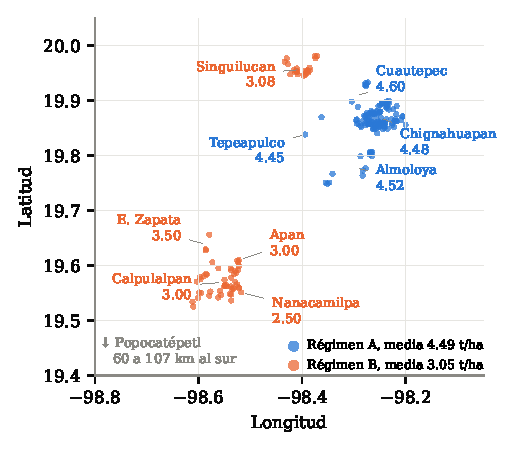
\includegraphics[width=\columnwidth]{r2_mapa}
\caption{Las 197 parcelas por régimen, con el rendimiento medio de entrenamiento de cada municipio. Singuilucan, de
régimen B, colinda con Cuautepec y Tepeapulco, de régimen A.}
\label{fig:mapa}
\end{figure}
